\section{Lucky Patcher} \label{section:luckypatcher-explain}
\begin{itemize}
  \item what is luckypatcher, what is written about it on the site, who created it
  \item lucky patcher is used to crack, remove ads and permissions
  \item works with and without root
  \item indirect patching without root
  \item root and busybox when direct patching
  \item requires no technical knowledge since automatic, popular
  \item focus on bypassing license verification, works as legally aquired
  \item does not attack server connection but application code
  \item how does applying a patch work, does not guarantee success
  \item analysed in two ways, code and cracked applications
\end{itemize}

\begin{figure}[h]
    \centering
    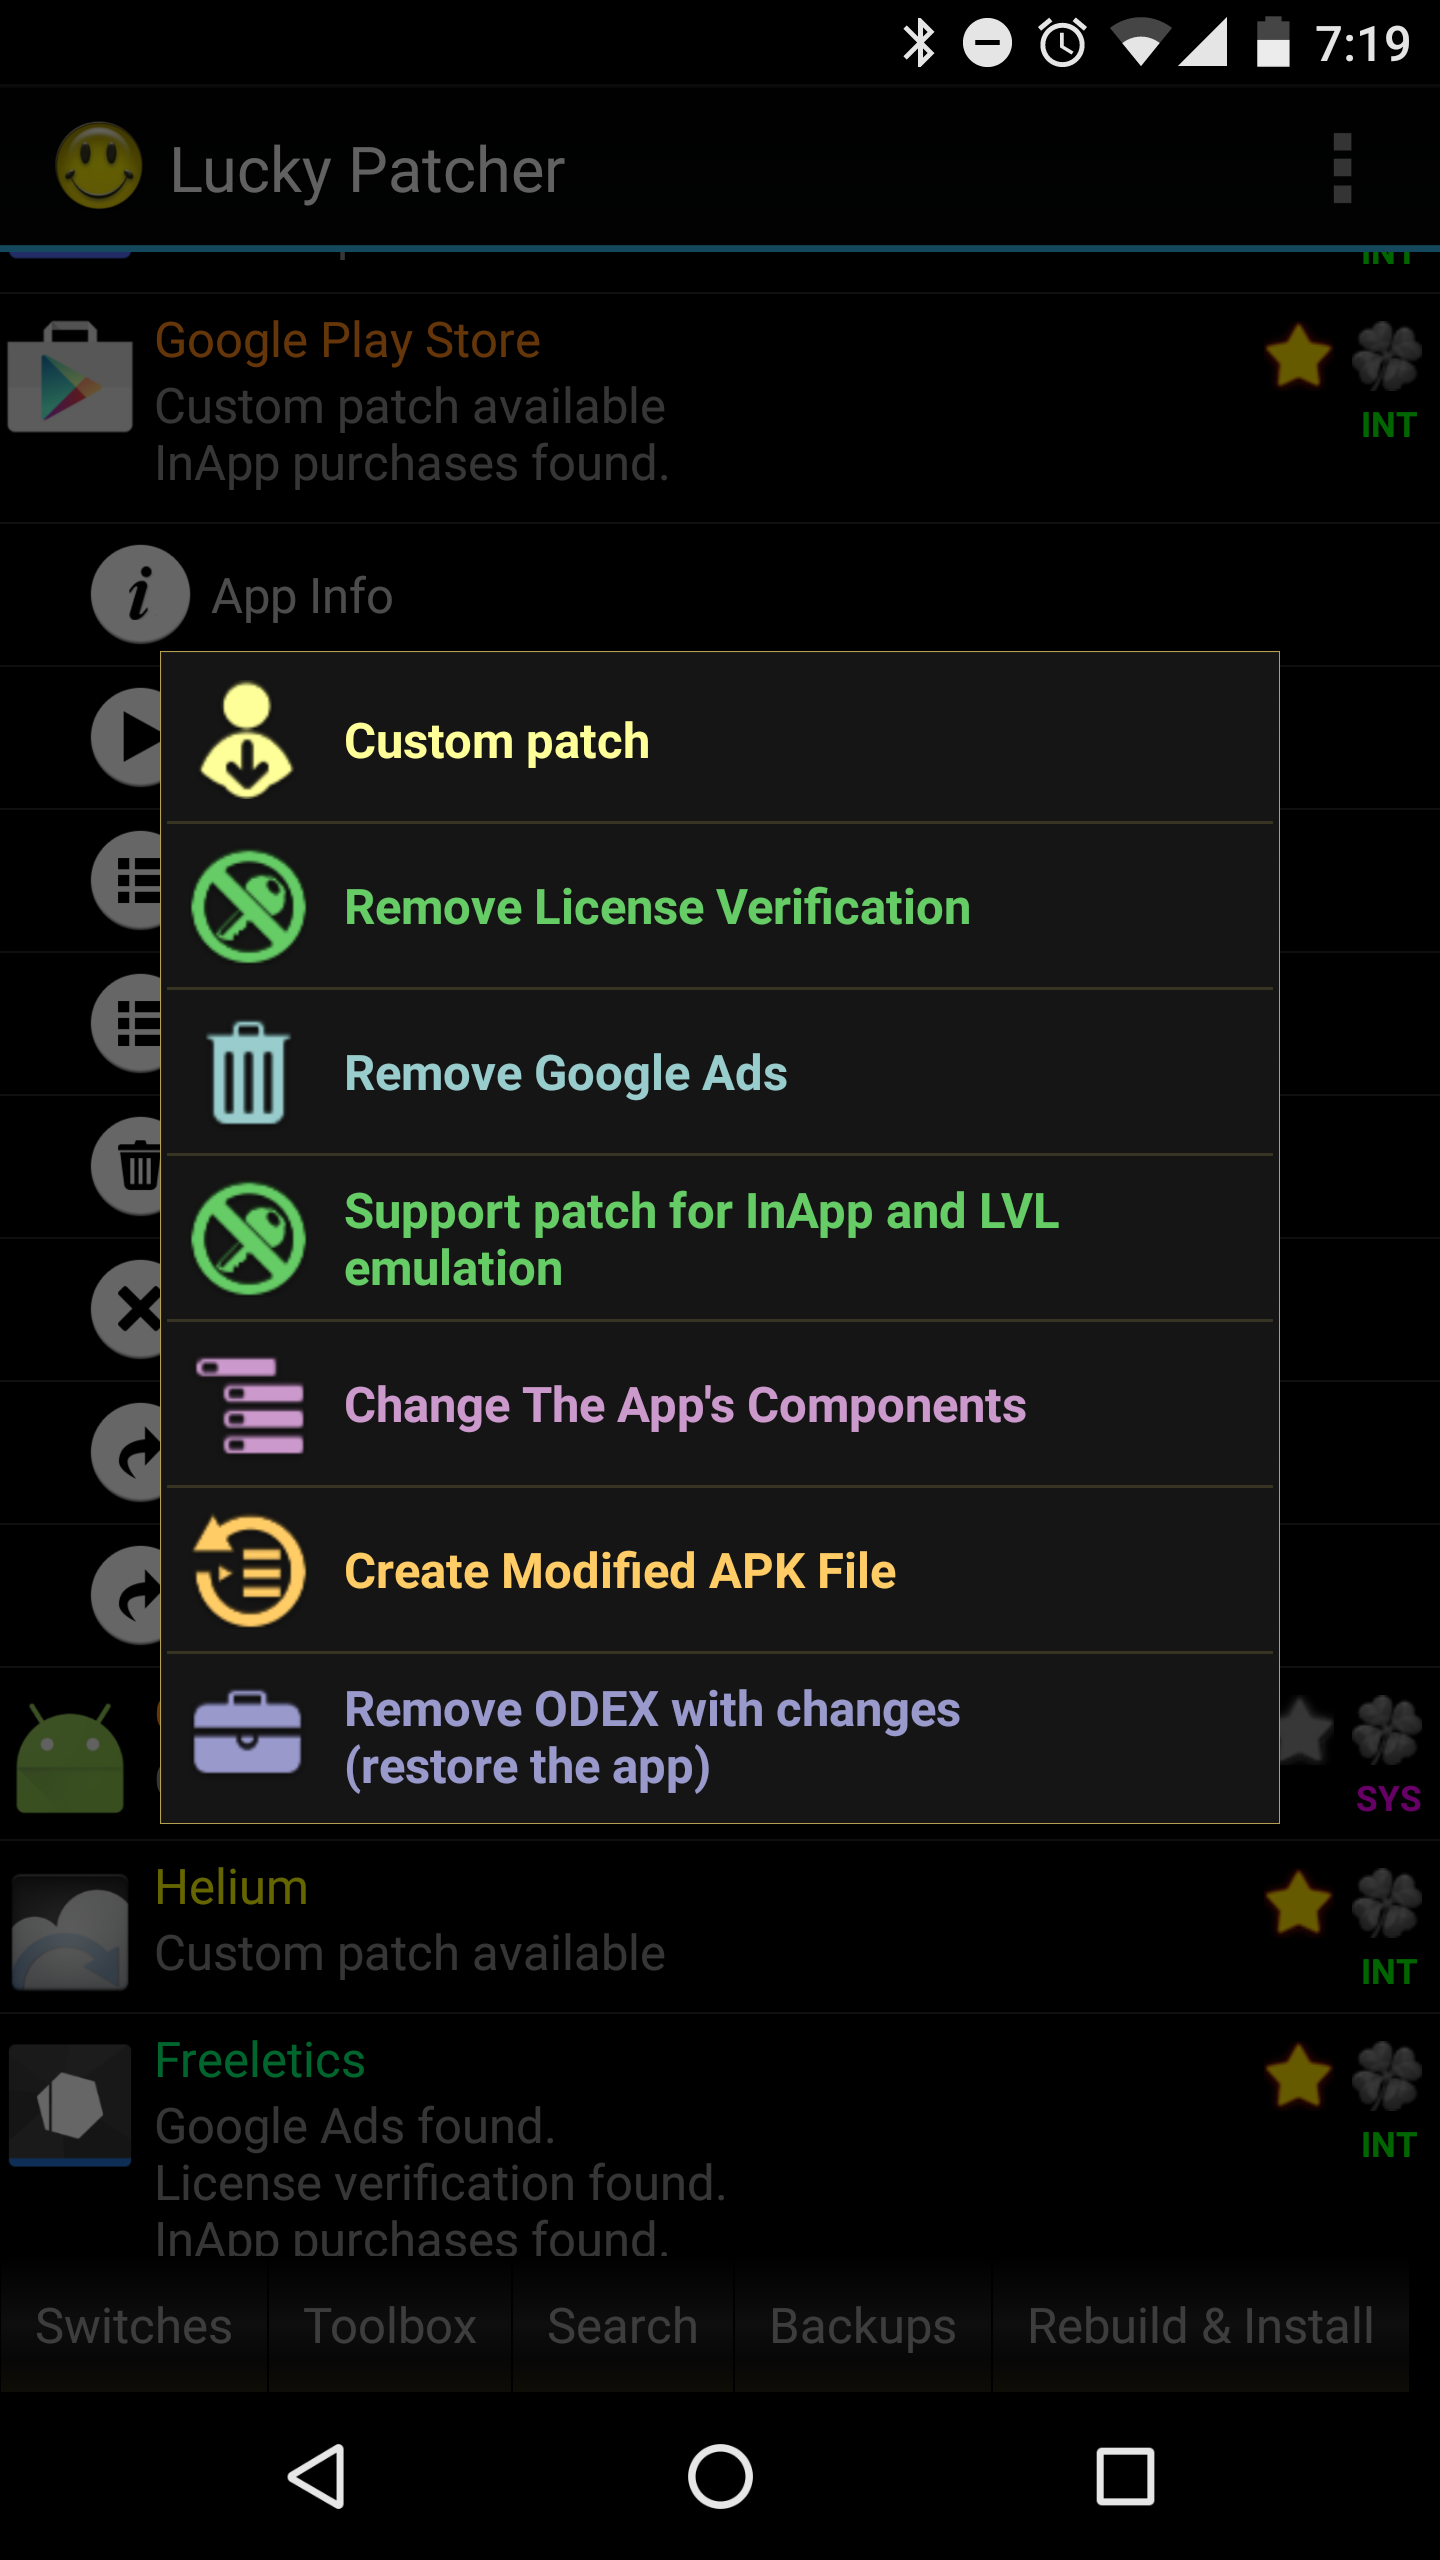
\includegraphics[width=0.3\textwidth]{data/luckyFeatures.png}
    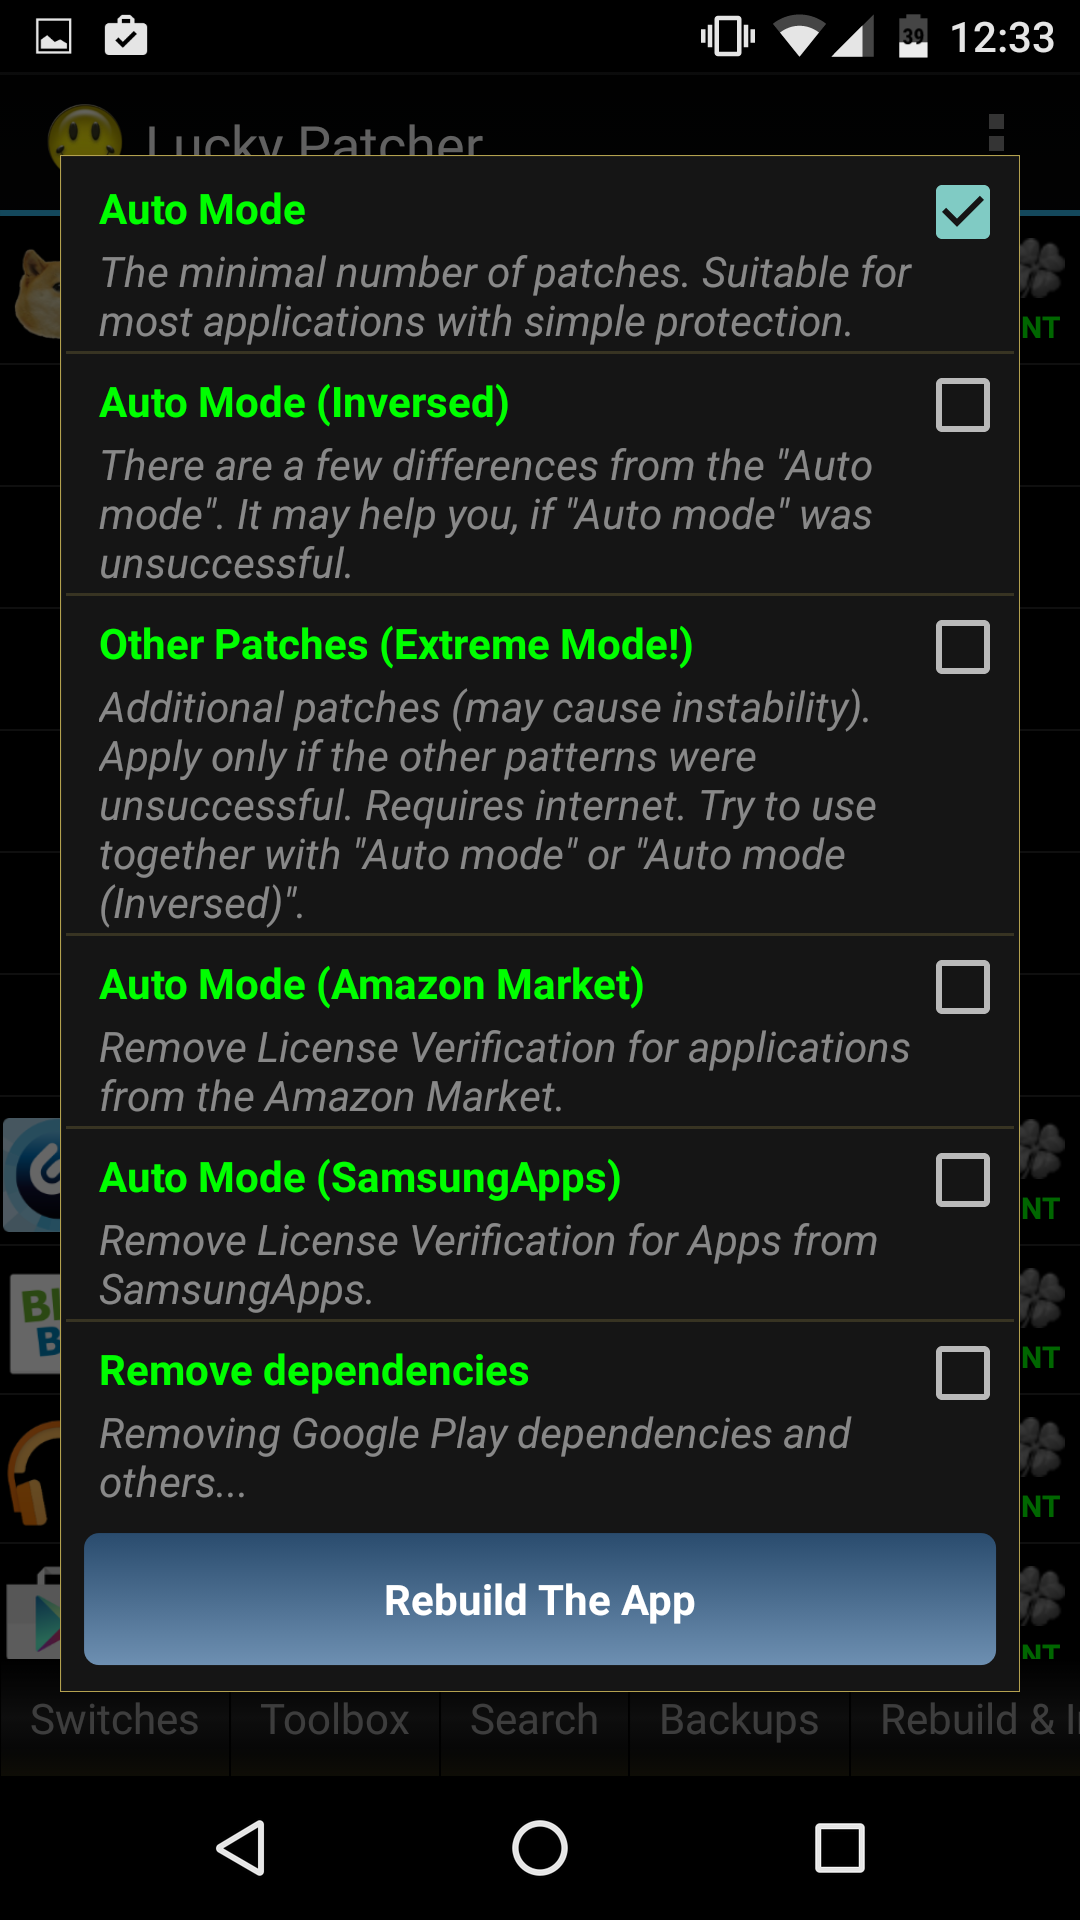
\includegraphics[width=0.3\textwidth]{data/luckyModi.png}
    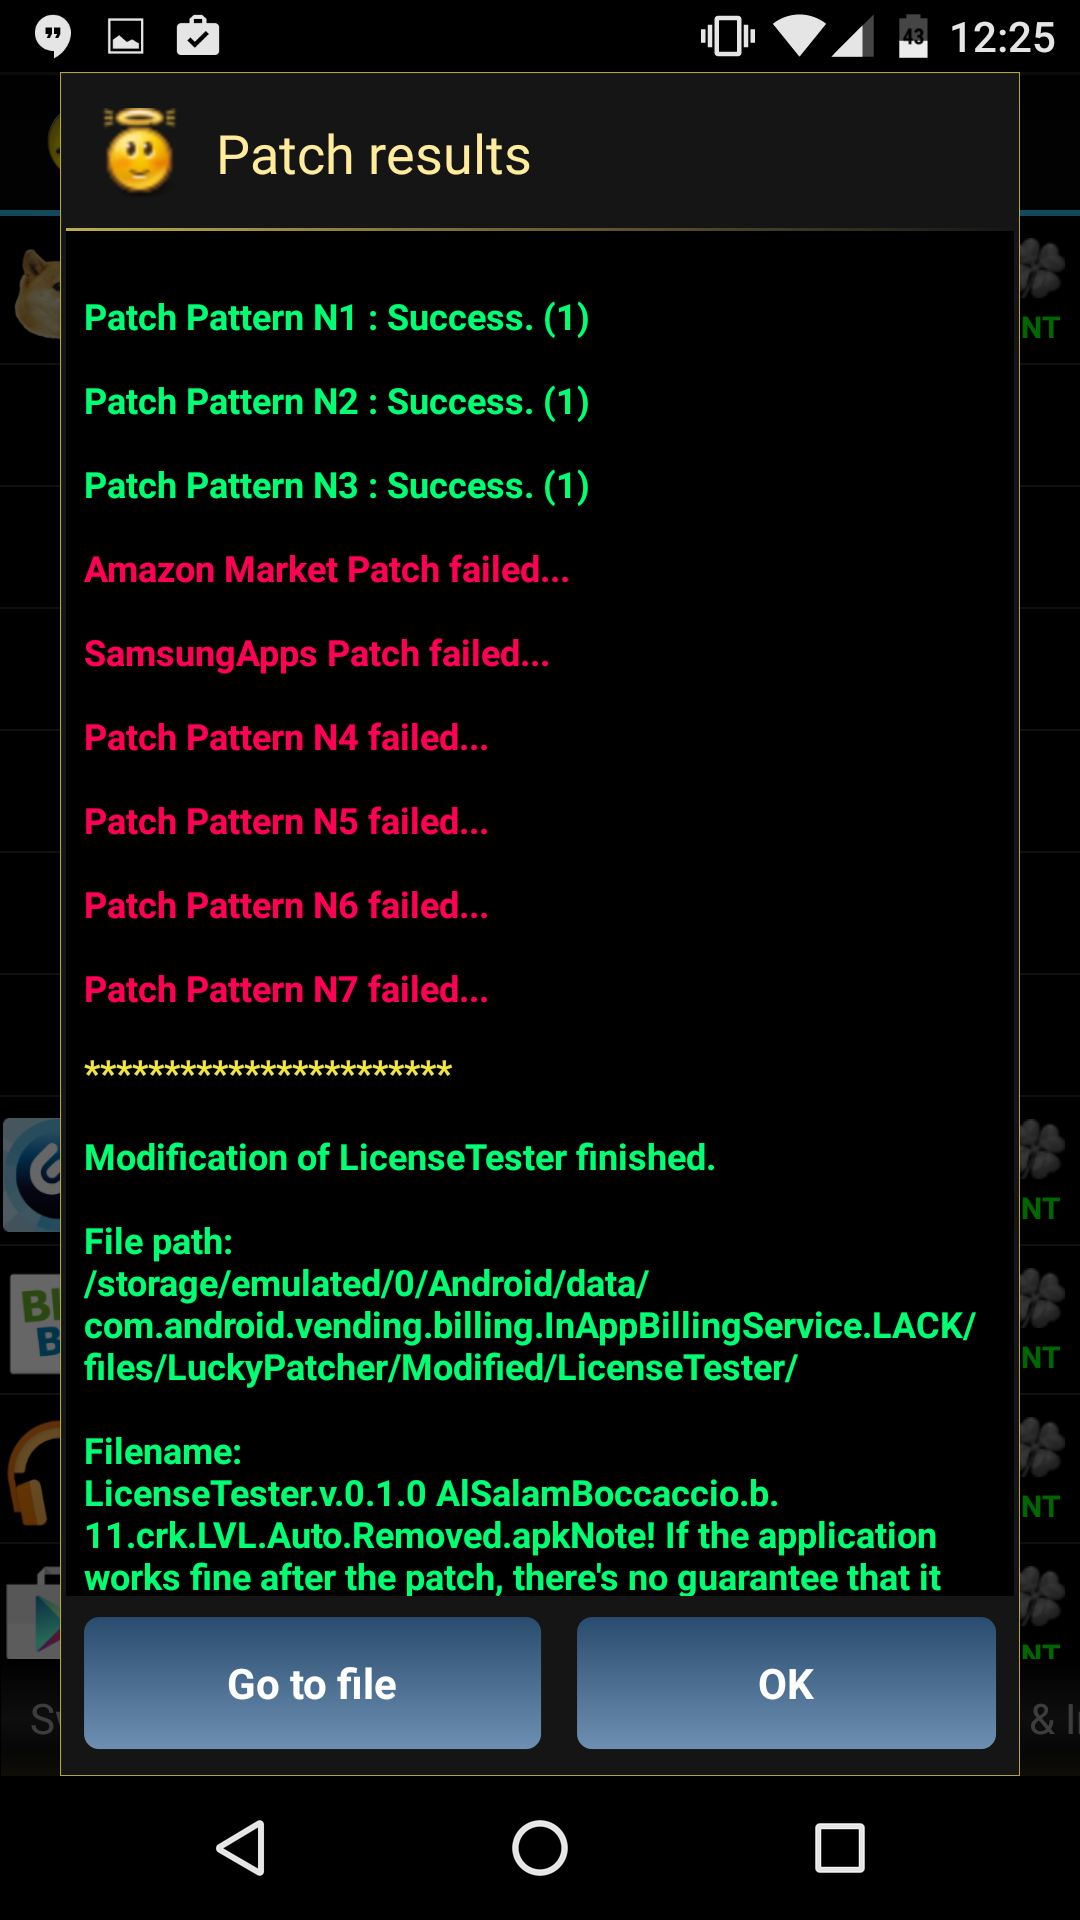
\includegraphics[width=0.3\textwidth]{data/luckyPatching.png}
    \caption{Left to right: Features offered LuckyPatcher, modes to crack license verification and the result after patching}
    \label{fig:luckyScreen}
\end{figure}
